\documentclass{beamer}

\usepackage{ucs}
\usepackage[utf8x]{inputenc}
\usepackage[T1]{fontenc}
\usepackage[english]{babel}
\usepackage[retainorgcmds]{IEEEtrantools}%	IEEEeqnarray
\usepackage{mathabx}%	convolution symbol
\usepackage{multi row}
\usepackage{epstopdf}
\usepackage{color}
\usepackage{listings}

\lstset{ %
language=C++,                % choose the language of the code
basicstyle=\scriptsize,       % the size of the fonts that are used for the code
numbers=left,                   % where to put the line-numbers
numberstyle=\scriptsize,      % the size of the fonts that are used for the line-numbers
stepnumber=1,                   % the step between two line-numbers. If it is 1 each line will be numbered
numbersep=5pt,                  % how far the line-numbers are from the code
showspaces=false,               % show spaces adding particular underscores
showstringspaces=false,         % underline spaces within strings
showtabs=false,                 % show tabs within strings adding particular underscores
tabsize=2,          % sets default tabsize to 2 spaces
captionpos=b,           % sets the caption-position to bottom
breaklines=true,        % sets automatic line breaking
breakatwhitespace=false,    % sets if automatic breaks should only happen at whitespace
}


\setbeameroption{show notes}

%	presentation info
\title{The Cilk Plus Extension}

\author{José Alves, Rui Brito}

\institute[pg22765, pg22781]{
	Universidade do Minho
}

\date{Braga, May 2013}


%	beamer options
\usetheme{Frankfurt}


\begin{document}%	begin presentation

\maketitle%	title slide

\begin{frame}
	\frametitle{Index}
	\tableofcontents
\end{frame}


\section{What is Cilk Plus}
\subsection{}
\begin{frame}
	\begin{block}{What is Cilk Plus}
			\begin{itemize}
				\item Intel Cilk Plus is an extension to the C and C++ languages to support task and data parallelism;
				\item As an extension implemented in the compiler it provides lower overhead than library-only solutions;
			\end{itemize}		
	\end{block}
\end{frame}

\subsection{}
\begin{frame}
	\begin{block}{Key Features}
			\begin{itemize}
				\item Keywords: cilk adds three new keywords to the C/C++ languages to better express task parallelism in an application;
				\item Reducers: a mechanism to eliminate contention for shared variables;
				\item \#pragma simd: a directive that tells the compiler a loop should be vectorized;
				\item Array Notations: a language addition to specify data parallelism for arrays or sections of arrays;  				
			\end{itemize}		
	\end{block}
\end{frame}

\section{The Cilk Plus Extension}
\subsection{}
\begin{frame}[fragile]
	\begin{block}{Keywords}	
		\begin{itemize}
			\item cilk\_spawn: tells the runtime environment that the statement following the cilk\_spawn keyword can be run in parallel with other statements;
			\item cilk\_sync: tells the runtime environment that all children of the spawning block must finish their execution before execution can continue;
			\item cilk\_for: a replacement for the standard C/C++ for loop that lets iterations run in parallel;
		\end{itemize}
	\end{block}
\end{frame}


\subsection{}
\begin{frame}[fragile]
	\begin{block}{cilk\_spawn example}	
		\begin{lstlisting}
			double fib(double n) {
    if (n < 2)
        return n;

    if (n < 30)
        return seq_fib(n);

    double x = cilk_spawn fib(n-1);
    double y = fib(n-2);
    cilk_sync;
    return x + y;
}
		\end{lstlisting}
	\end{block}
\end{frame}



\subsection{}
\begin{frame}[fragile]
	\begin{block}{cilk\_for example}	
		\begin{lstlisting}
		float* matrixDot (float *a, float *b, int n) {
			
			float value = 0;
			float *res = (float*) malloc(n * n * sizeof(float));

			cilk_for (int i = 0; i < n; ++i) {
				for(int j = 0; j < n; ++j) {			
					for(int k = 0; k < n; ++k) {
							value += a[i * n + k] * b[k * n + j];
					}
					res[i * n + j] = value;
					value = 0;
				}
			}
			
			
			return res;

		}
		\end{lstlisting}
	\end{block}
\end{frame}

\subsection{}
\begin{frame}
	\begin{block}{More on cilk\_for}
		\begin{itemize}
			\item Using cilk\_for is not the same as spawning each loop iteration.
			\item The compiler converts the loop body to a function that is called recursively using a divide-and-conquer strategy;
		\end{itemize}
	\end{block}
\end{frame}

\subsection{}
\begin{frame}
		\begin{figure}[!htb]
			\centering
			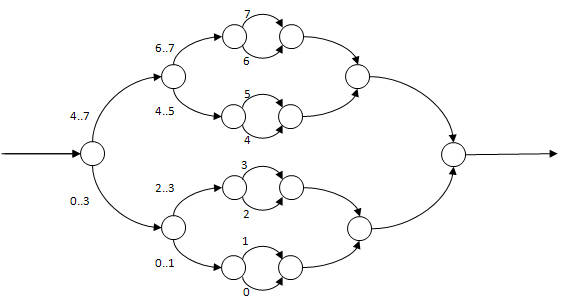
\includegraphics[scale=1]{images/cilkfor.jpg}
			\caption{cilk\_for with N=8 iterations}
			\label{roofline}
		\end{figure}

\end{frame}

\subsection{}
\begin{frame}[fragile]
	\begin{block}{Reducers}					
		\begin{lstlisting}
			void reducer_list_test() {
    cilk::reducer_list_append<char> letters_reducer;

    cilk_for(char ch = 'a'; ch <= 'z'; ch++){
        simulated_work();
        letters_reducer.push_back(ch);
    }

    const std::list<char> &letters = letters_reducer.get_value();

    for(std::list<char>::const_iterator i = letters.begin(); i != letters.end(); i++) {
        std::cout << " " << *i;
    }
    std::cout << std::endl;
}
		\end{lstlisting}
	\end{block}
\end{frame}

\scriptsize

\subsection{}
\begin{frame}[fragile]
	\begin{block}{Available reducers}
		\begin{itemize}
			\item reducer\_list\_append: Creates a list by adding elements to the back;
			\item reducer\_list\_prepend: Creates a list by adding elements to the front;
			\item reducer\_max: Calculates the maximum value of a set of values;
			\item reducer\_max\_index: Calculates the maximum value and index of that value of a set of values;
			\item reducer\_min: Calculates the minimum value of a set of values;
			\item reducer\_min\_index: Calculates the minimum value and index of that value of a set of values;
			\item reducer\_opadd: Calculates the sum of a set of values;
			\item reducer\_opand: Calculates the binary AND of a set of values;
			\item reducer\_opor: Calculate the binary OR of a set of values;
			\item reducer\_opxor: Calculate the binary XOR of a set of values;
			\item reducer\_string: Accumulates a string using append operations;
			\item reducer\_wstring: Accumulates a "wide" string using append operations;
			\item reducer\_ostream: An output stream that can be written in parallel;
			\item reducer\_ostream: An output stream that can be written in parallel;
		\end{itemize}
	\end{block}
\end{frame}

\normalsize

\subsection{}
\begin{frame}[fragile]
	\begin{block}{Array Notation}
		\begin{itemize}
			\item An array section assignment is a parallel operation that modifies every element of the array section on the left-hand side;
			\item Makes uses of vectorization techniques;
			\item Explicit high-level mechanism for expressing SIMD instructions (explicit \#pragma simd);			
		\end{itemize}
	\end{block}
\end{frame}


\subsection{}
\begin{frame}[fragile]
	\begin{block}{Examples}
		\begin{lstlisting}
			// Copy elements 10->19 in A to elements 0->9 in B.
B[0:10] = A[10:10];
// Transpose row 0, columns 0-9 of A, into column 0, rows 0-9 of B.
B[0:10][0] = A[0][0:10];
// Copy the specified array section in the 2nd and 3rd dimensions of A into the 1st and 4th dimensions of B.
B[0:10][0][0][0:5] = A[3][0:10][0:5][5]
// Set all elements of A to 1.0.
A[:] = 1.0;
// Add elements 10->19 from A with elements 0->9 from B and place in elements 20->29 in C.
C[20:10] = A[10:10] + B[0:10];
// Element-wise equality test of B and C, resulting in an array of Boolean values, which are placed in A.
A[:] = B[:] == C[:];
		\end{lstlisting}
	\end{block}
\end{frame}

\subsection{}
\begin{frame}[fragile]
	\begin{block}{Scheduler}
		\begin{itemize}
			\item The Cilk Plus runtime uses a work-stealing scheduler to dynamically load-balance the tasks that are created by a Cilk Plus program;
			\item At a high level, the runtime scheduler executes a Cilk Plus program by using worker threads;
			\item In runtime, each worker thread maintains its deque using the following simple algorithm:
			\begin{itemize}
				\item When a worker thread executes a cilk\_spawn or a cilk\_for statement, it may push new tasks onto the tail of its deque.
				\item When a worker thread reaches a cilk\_sync that needs to wait for a spawned function to complete, it tries to keep busy by popping a task from the tail of its deque.
				\item If the worker thread discovers that its deque is empty, it tries to steal work from the head of the deque of another worker, where the worker is chosen at random.
			\end{itemize}
		\end{itemize}
	\end{block}
\end{frame}

\section{Cilk vs OpenMP}
\subsection{}
\begin{frame}
		\begin{figure}[!htb]
			\centering
			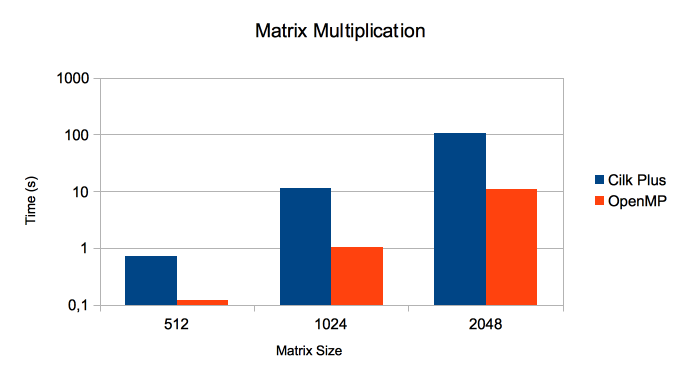
\includegraphics[scale=0.45]{images/matrix.png}
			\caption{Results for matrix multiplication}
			\label{roofline}
		\end{figure}
\end{frame}

\subsection{}
\begin{frame}
		\begin{figure}[!htb]
			\centering
			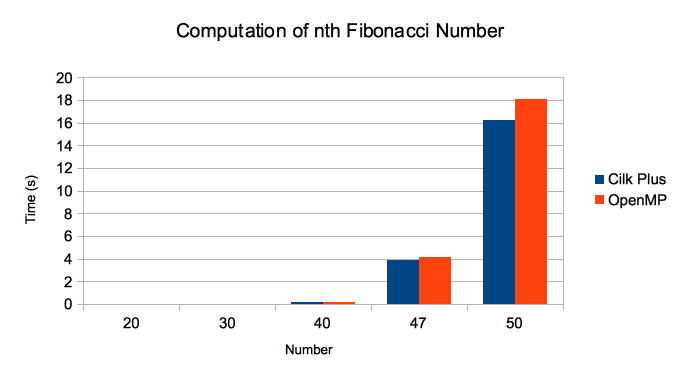
\includegraphics[scale=0.45]{images/fib.png}
			\caption{Results for fibonacci computation}
			\label{roofline}
		\end{figure}
\end{frame}

\subsection{}
\begin{frame}
		\begin{figure}[!htb]
			\centering
			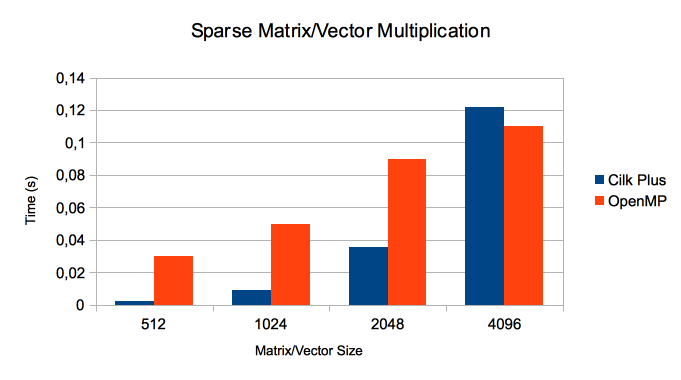
\includegraphics[scale=0.45]{images/sparse.png}
			\caption{Results for sparse matrix/vector multiplication}
			\label{roofline}
		\end{figure}
\end{frame}

\subsection{}
\begin{frame}
		\begin{figure}[!htb]
			\centering
			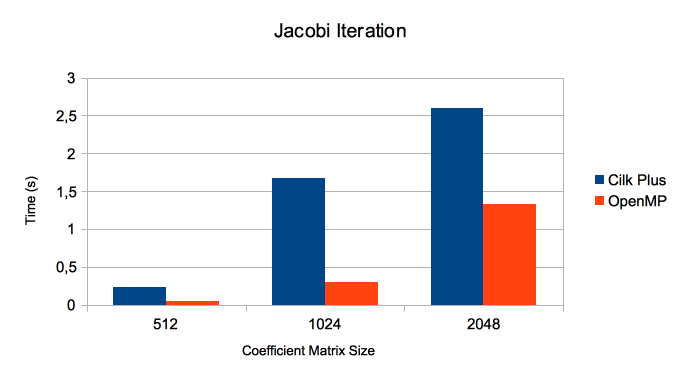
\includegraphics[scale=0.45]{images/jacobi.png}
			\caption{Results for jacobi iteration}
			\label{roofline}
		\end{figure}
\end{frame}

\section{Conclusion}
\begin{frame}[fragile]
	\begin{block}{Conclusions}
		\begin{itemize}
			\item Ease of use makes it a powerful competitor;			
			\item Not as powerful as OpenMP (although it can work together with TBB);
			\item Good for recursive algorithms;
			\item Spawning threads has very low overhead;
			\item Automatic load balancing is a plus;
			\item Supports incremental parallelization;		
		\end{itemize}		
	\end{block}
\end{frame}


\section{Questions}
\begin{frame}
\titlepage
	\begin{center}
		\Huge\bfseries
		- ? -
	\end{center}
\end{frame}

\end{document}%	end presentation